% ########################################################################################################################################
%
% This is the main latex file. Here we call for inputs from other files. We also define some of the main characteristics of the document.
%
% ########################################################################################################################################
%
% You likely only need to modify the "Main_Content__Write_your_essay_here.tex" file.
%
% ########################################################################################################################################

\documentclass[12pt,a4paper,oneside]{paper}
%TC:ignore
% ################################################################################
% 
%       INSTRUCTIONS, PLEASE READ BEFORE IF YOU INTEND TO MODIFY THIS FILE
% 
% ################################################################################
% For the most part, you should not change this file. In particular, the format 
% should not be changed. However, depending on what you want you might need to
% use additional packages (and possibly remove old ones that may be incompatible.
% Do that at your own discretion.
% ################################################################################

% Encoding and Language
\usepackage[utf8x]{inputenc}
\usepackage{csquotes}
\usepackage[main=portuguese]{babel}
\usepackage{iflang}

% Font Configurations
\renewcommand{\rmdefault}{phv}
\renewcommand{\sfdefault}{phv}
\def\FontLn{% 16 pt normal
  \usefont{T1}{phv}{m}{n}\fontsize{14pt}{14pt}\selectfont}
\def\FontLb{% 16 pt bold
  \usefont{T1}{phv}{b}{n}\fontsize{14pt}{14pt}\selectfont}
\def\FontMn{% 14 pt normal
  \usefont{T1}{phv}{m}{n}\fontsize{12pt}{12pt}\selectfont}
\def\FontMb{% 14 pt bold
  \usefont{T1}{phv}{b}{n}\fontsize{12pt}{12pt}\selectfont}
\def\FontSn{% 12 pt normal
  \usefont{T1}{phv}{m}{n}\fontsize{10pt}{10pt}\selectfont}

% Font Encoding
\usepackage[T1]{fontenc}

% Page Geometry
\usepackage{geometry}	
\geometry{verbose,tmargin=2cm,bmargin=1.7cm,lmargin=2cm,rmargin=2cm}
\usepackage{multirow}
\usepackage{multicol}

% Line Spacing
\usepackage{setspace}
\renewcommand{\baselinestretch}{1.2}

% Graphics and Figures
\usepackage{graphicx}
\usepackage{subfigure}
\usepackage{subfigmat}
\usepackage{float}

%Colors
\usepackage{xcolor}

% Mathematics and Theorems
\usepackage{amsmath}
\usepackage{amsthm}
\usepackage{amsfonts}
\usepackage{dcolumn}
\usepackage{indentfirst}

% Comments and Verbatim
\usepackage{verbatim}

% Hyperlinks
\usepackage[pdftex]{hyperref}
\hypersetup{
    colorlinks,
    linkcolor=blue,
    anchorcolor=black,
    citecolor=cyan,
    filecolor=black,
    menucolor=black,
    urlcolor=teal,
    bookmarksopen=true,
    bookmarksnumbered=true
}

% Captions and References
\usepackage[figure,table]{hypcap}
\usepackage[format=plain]{caption}
\DeclareCaptionFont{georgia}{\small\fontseries{n}\fontfamily{georgia}\selectfont}
\captionsetup{labelfont=georgia,font=georgia}

% Bibliography
\usepackage[backend=biber,style=apa]{biblatex}

% Index
\usepackage{makeidx}
\makeindex

% Acronyms
\usepackage[printonlyused]{acronym}

% Lipsum (for placeholder text)
\usepackage{lipsum}

% Cleveref (for clever references)
\usepackage[\IfLanguageName{english}{english}{portuguese}]{cleveref}

% Colors
\usepackage{xcolor}
\usepackage{color}

% Custom Commands
\newcommand{\gray}[1]{\textcolor{gray}{#1}}

% Equation Numbering
\renewcommand{\theequation}{{\fontseries{n}\fontfamily{georgia}\selectfont\arabic{equation}}}

% Section and Subsection Fonts
\sectionfont{\Large\bfseries\fontfamily{lmss}\selectfont}
\subsectionfont{\large\bfseries\fontfamily{lmss}\selectfont}
%TC:endignore


\addbibresource{bibliography.bib}
\begin{document}
\pagestyle{plain}

%TC:ignore
% #############################################################################
%
%                           ENTER YOUR NAME, ISTid, AND TITLE
% 
% #############################################################################



\def\title {Velocidade da Luz}


% #############################################################################
%
%               DO NOT MODIFY THE LINES FROM HERE TO THE MAIN DOCUMENT BODY
% 
% #############################################################################

\thispagestyle {empty}
\begin{center}
\begin{minipage}[c][5cm][t]{\textwidth}
\begin{center}

\includegraphics[width=5cm]{../IST_A_RGB_POS.png}
\end{center}

\end{minipage}
\begin{minipage}[t][10cm][c]{\textwidth}
\centering
{\FontMb Instituto Superior Técnico} \\
\paragraph{}
\centering
{\FontLb\Huge \title{}}
\paragraph{}
\centering
{\FontMb Laboratório de Introdução à Física Experimental} \\
\paragraph{}
{\FontMb 2023/2024}
\end{minipage}

\begin{minipage}[c][2cm][c]{\textwidth}
\centering
{\FontLn }
\end{minipage}
\begin{minipage}[c][2cm][c]{\textwidth}
\centering
\end{minipage}
\begin{minipage}[c][1cm][c]{\textwidth}
\centering
\fbox{{\FontMb Report}}
\end{minipage}
\begin{minipage}[c][3cm][c]{\textwidth}
\centering
{\FontMb
102716 Pedro Curvo}
\end{minipage}
\begin{minipage}[c][2cm][c]{\textwidth}
\centering

\end{minipage}

\end{center} 
\cleardoublepage
\fontfamily{cmr}\selectfont
\setcounter{page}{0}
%TC:endignore
% #############################################################################
%
%                           BEGIN MAIN DOCUMENT BODY
%
% #############################################################################

% -----------------------------------------------------------------------------
%                   Primeira Parte 
% -----------------------------------------------------------------------------
\section{Report}
Nesta atividade experimental, procedeu-se à substituição das lentes e da calha utilizada para montar a experiência,
devido às instabilidades observadas com a calha anterior. Optou-se por uma calha de precisão em alumínio triangular, utilizando
os suportes correspondentes para assegurar uma montagem sólida.

A introdução dessa nova calha, aliada aos suportes apropriados, resultou numa significativa melhoria na estabilidade do sistema ótico,
eliminando oscilações notáveis durante a execução da experiência. Vale destacar que, com esta calha, as distâncias marcadas
são representadas por números inteiros.

Quanto às lentes, foram substituídas por outras cujos suportes possibilitam um alinhamento mais fácil, permitindo ajustes
em três graus de liberdade: eixo X, Y e Z. Anteriormente, a alteração estava limitava à altura e à inclinação da lente,
tornando o alinhamento mais desafiador. A expetativa, com esta alteração, é que, mesmo diante de desalinhamentos durante a atividade,
os alunos tenham maior facilidade em corrigi-los.

Para além destes aspetos, o guia desta atividade experimental não foi alterado, sendo que apenas o material foi
substituído. A teoria e o procedimento experimental permanecem os mesmos, assim como as questões colocadas no final do guia.
A única alteração foi a substituição das imagens do guia que mostravam a experiência com a calha anterior, por imagens
da experiência com a nova calha. Contudo, estas imagens deverão ser posteriormente alteradas aquando da decisão do 
uso ou não deste material.

\section{Imagens}

\begin{figure}[H]
    \centering
    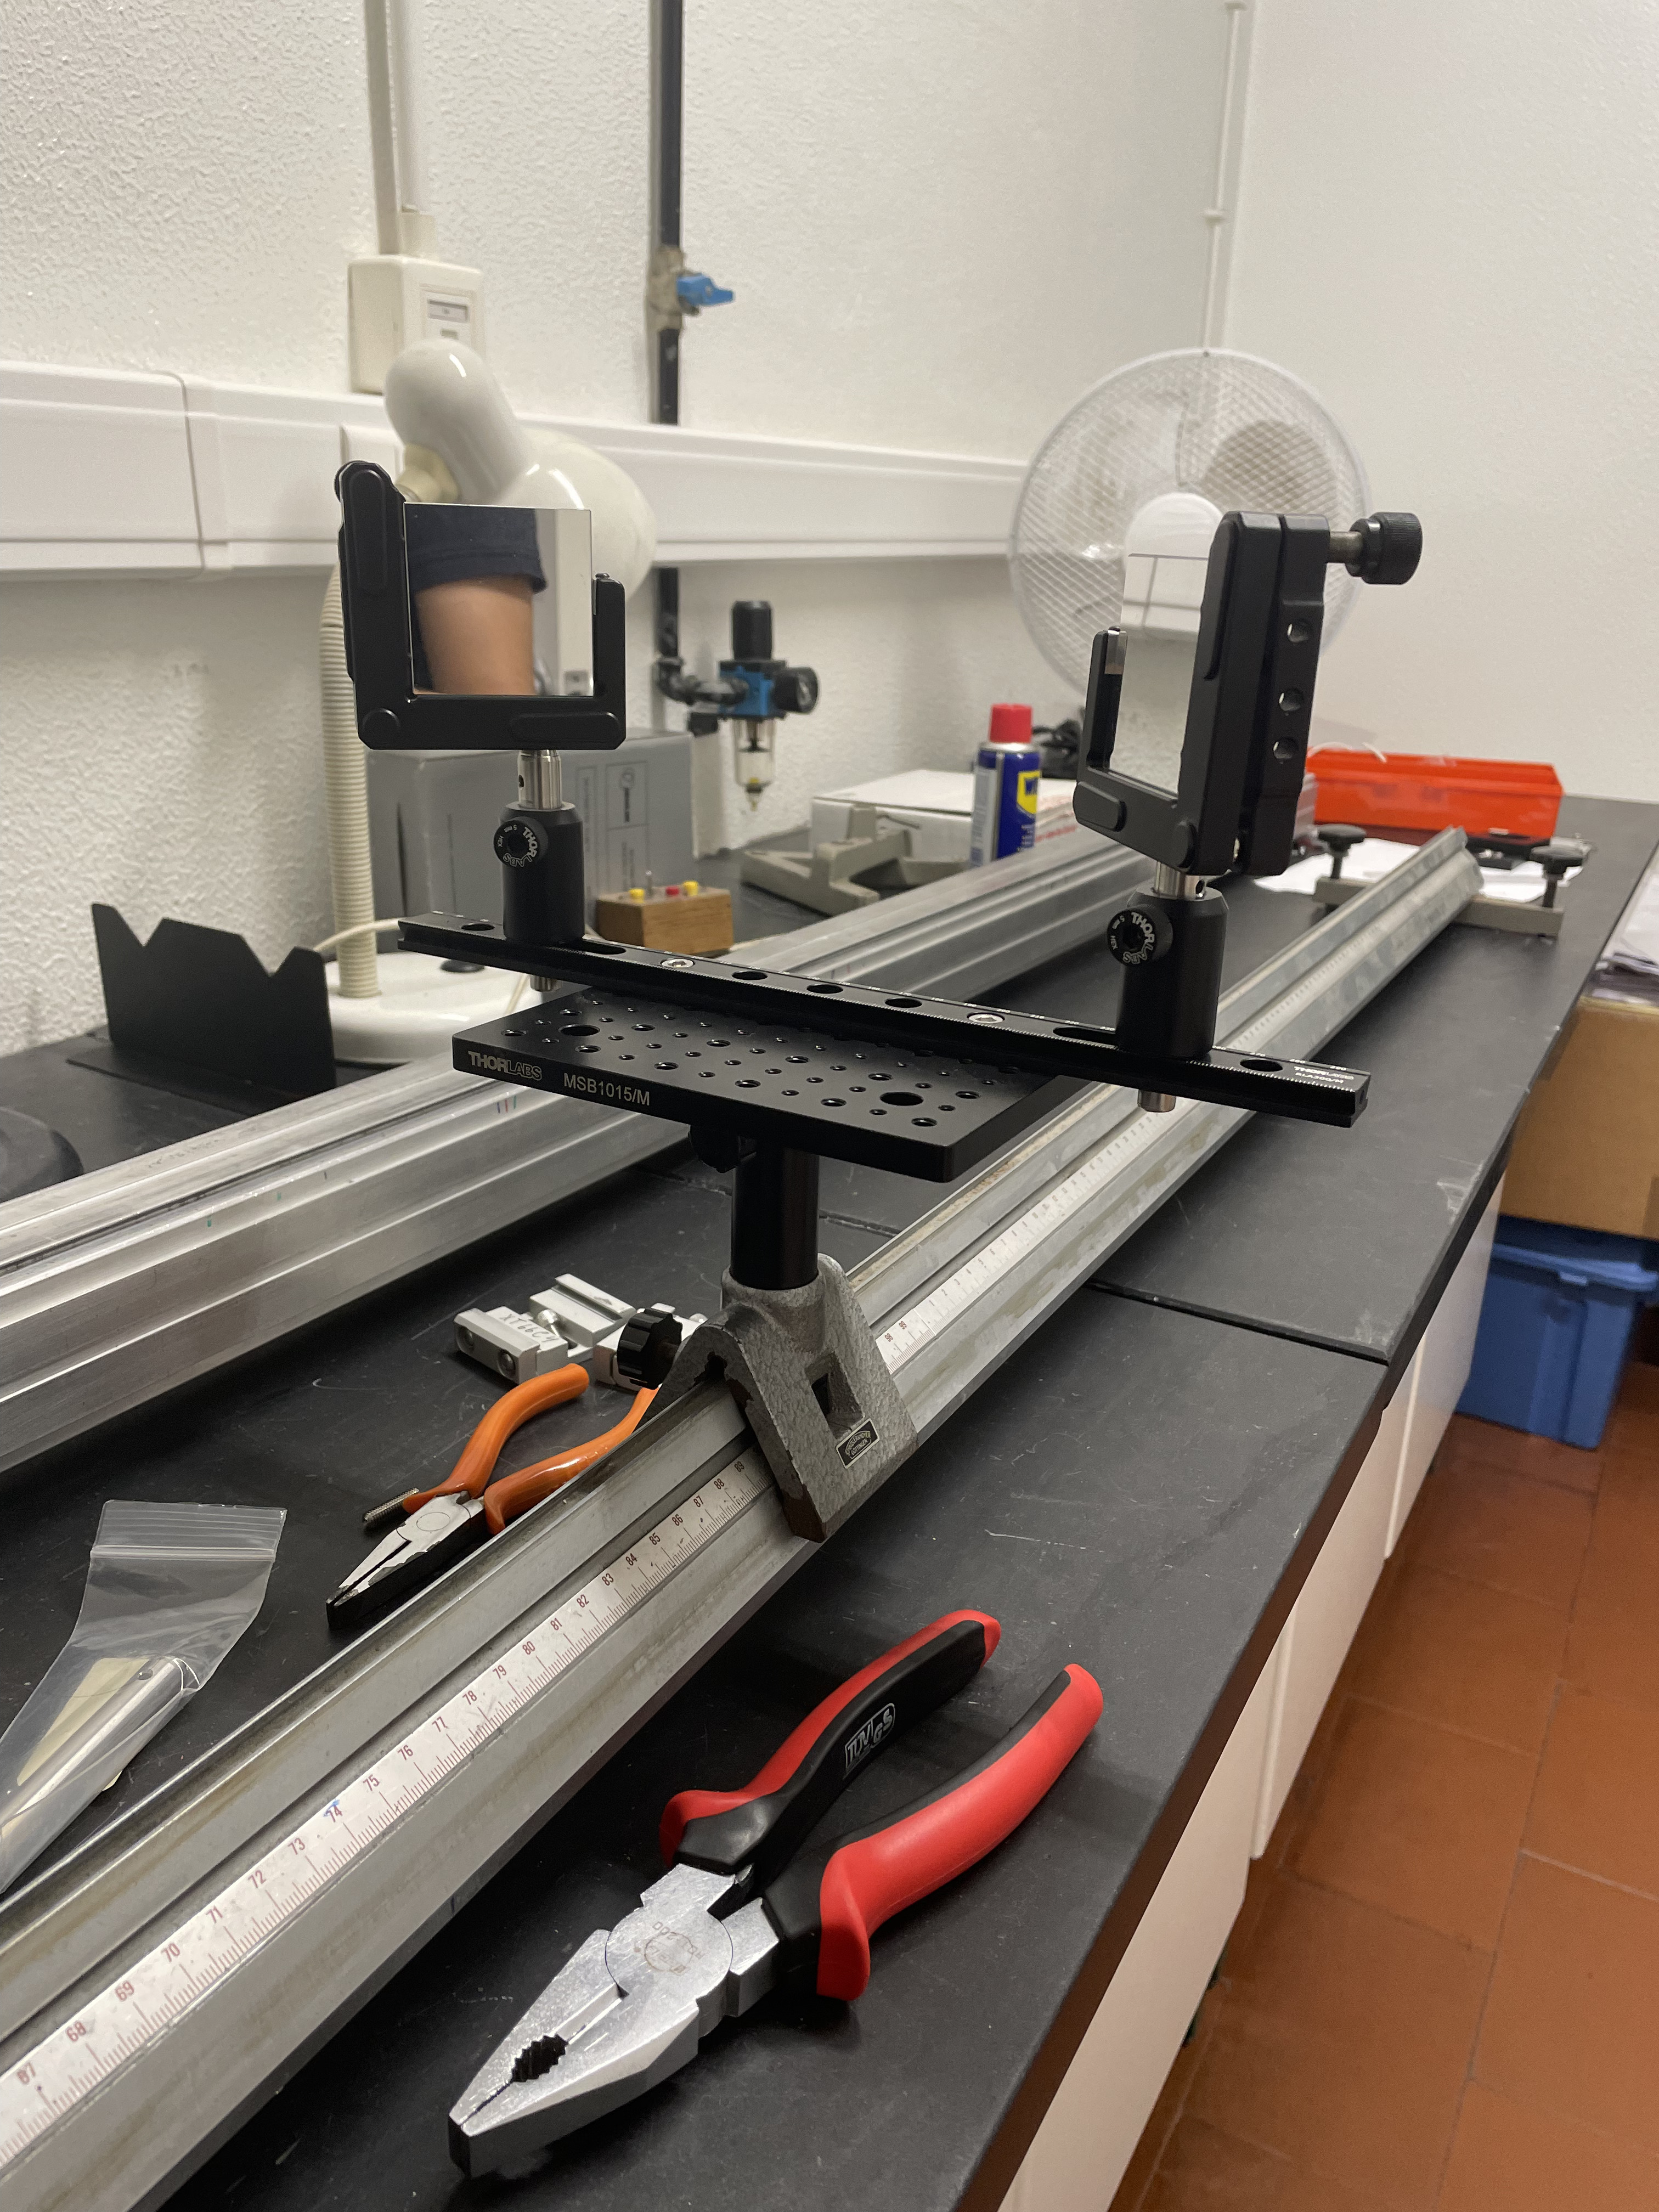
\includegraphics[width=0.6\textwidth]{IMG_2862.jpg}
    \caption{Montagem da experiência com a nova calha e as novas lentes.}
    \label{fig:montagem}
\end{figure}

\begin{figure}[H]
    \centering
    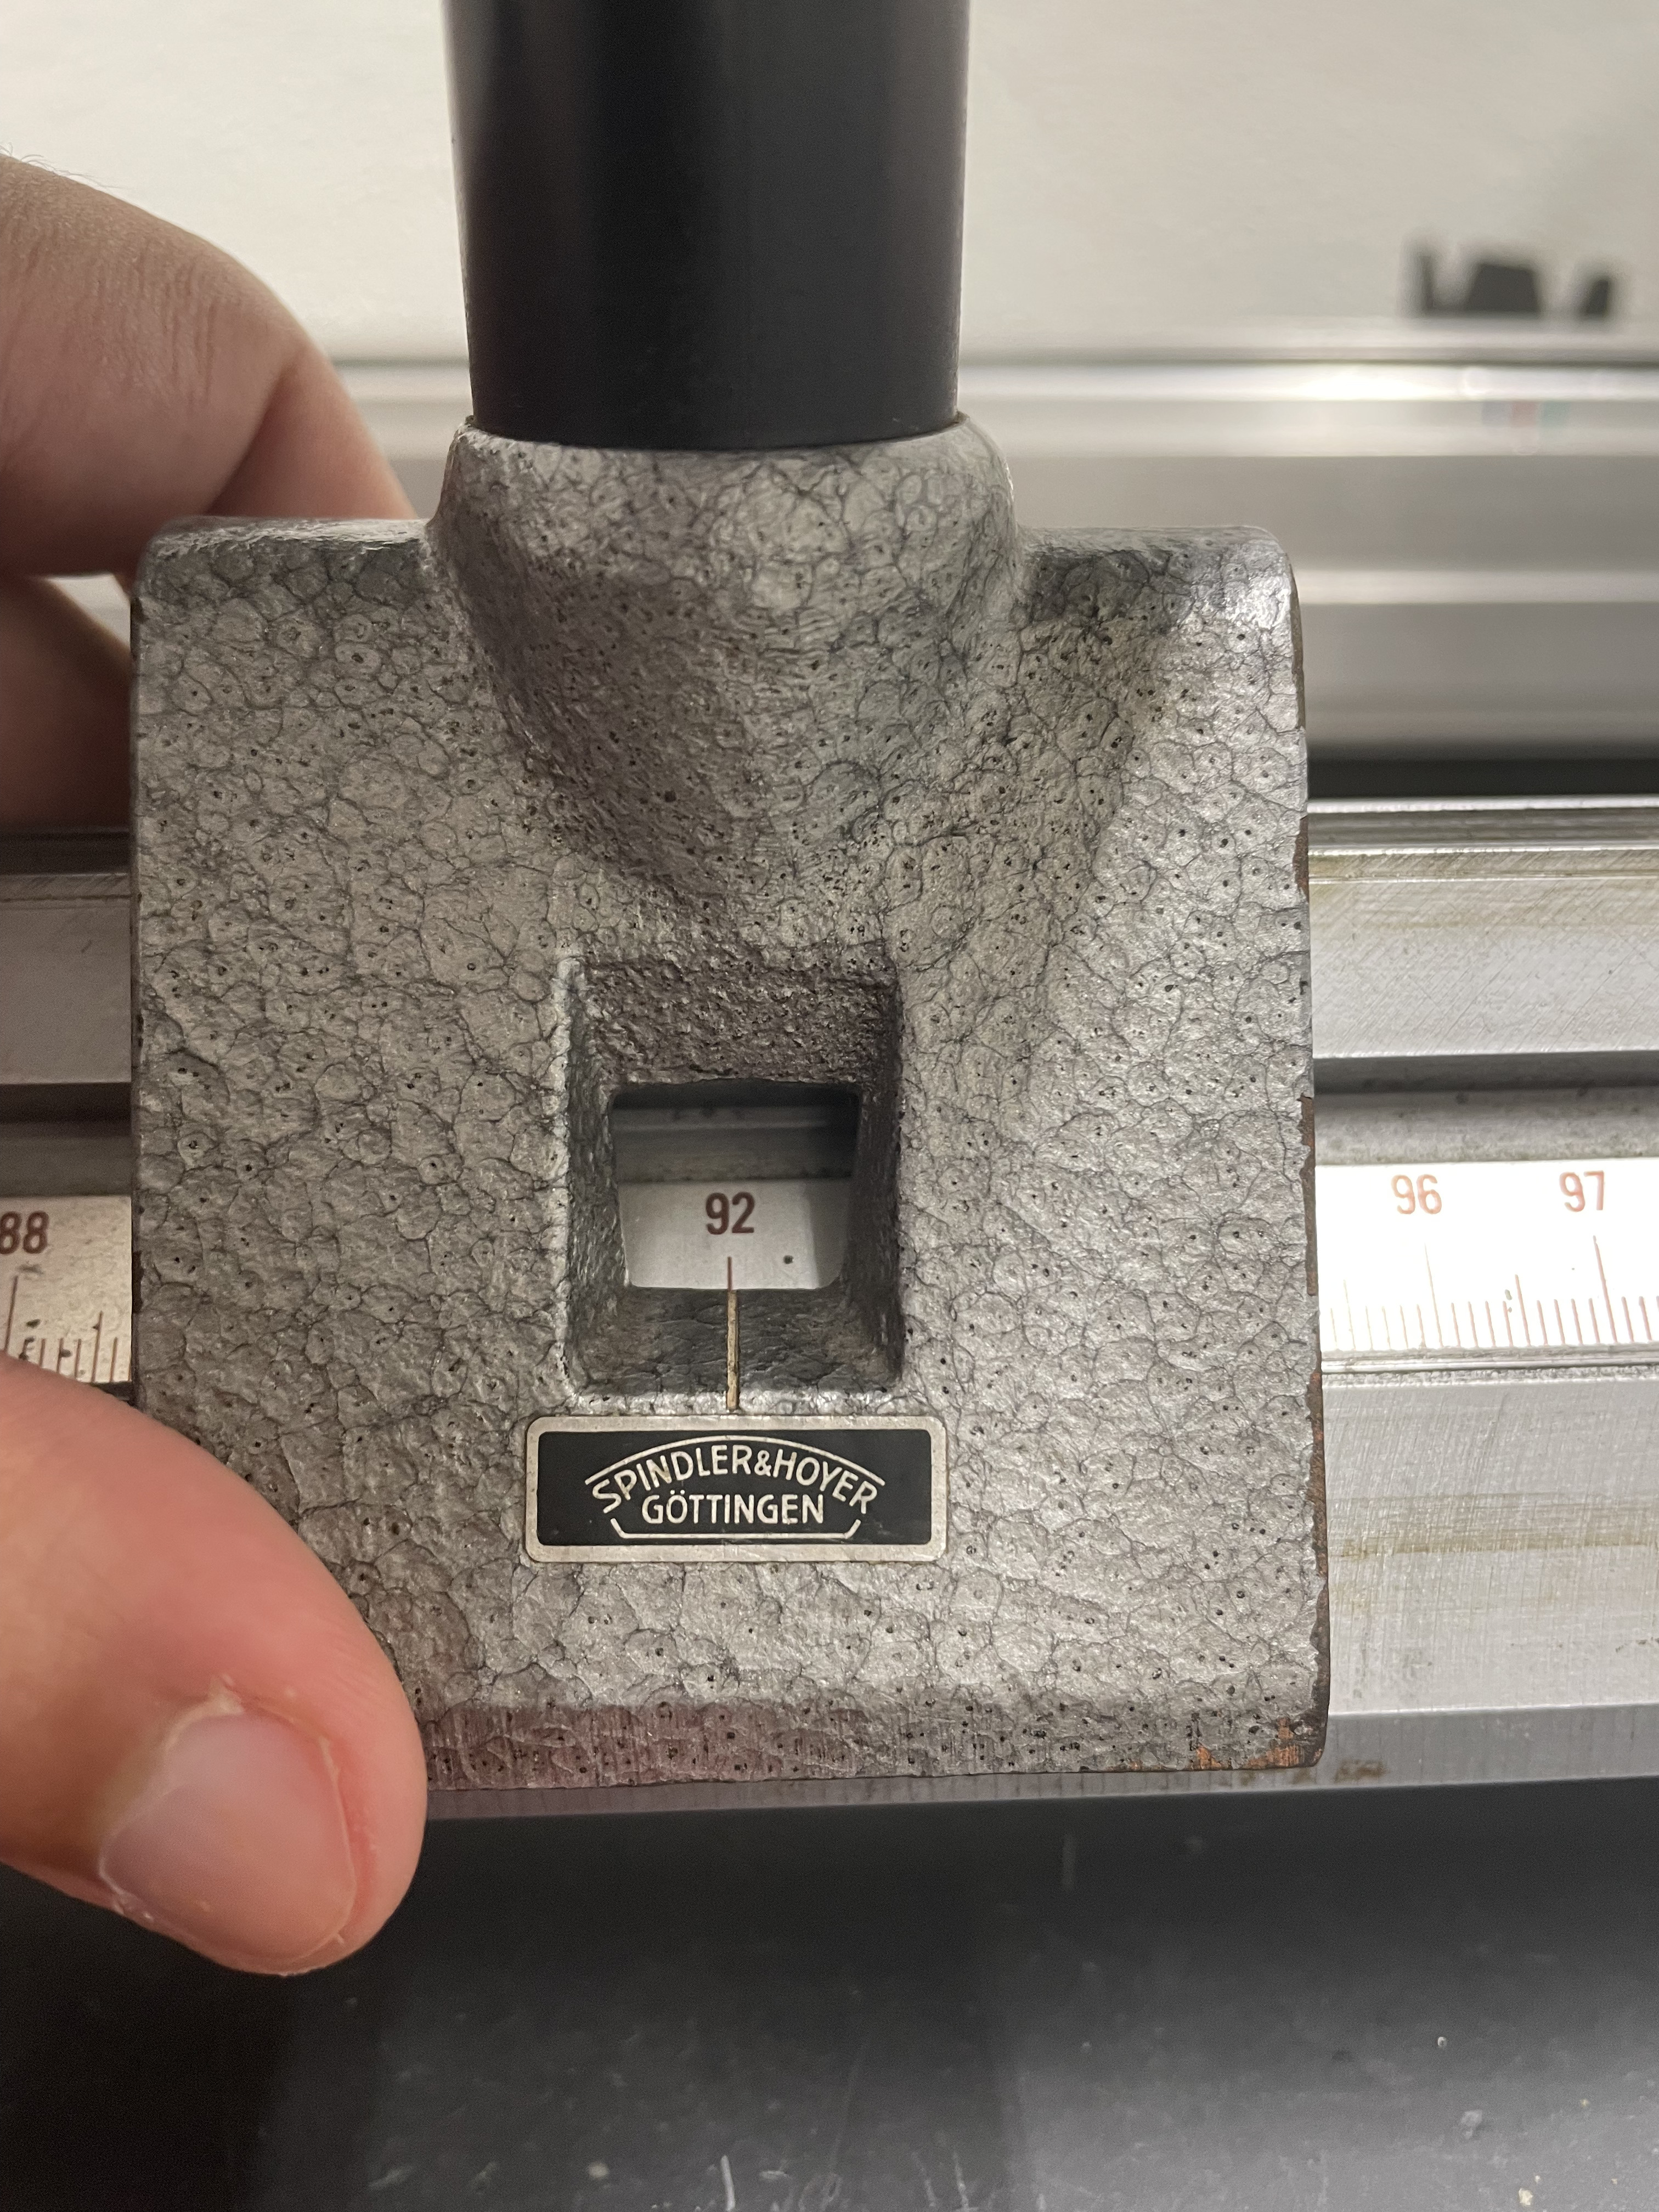
\includegraphics[width=0.6\textwidth]{IMG_2863.jpg}
    \caption{Montagem da experiência com a nova calha e as novas lentes.}
    \label{fig:montagem}
\end{figure}

\begin{figure}[H]
    \centering
    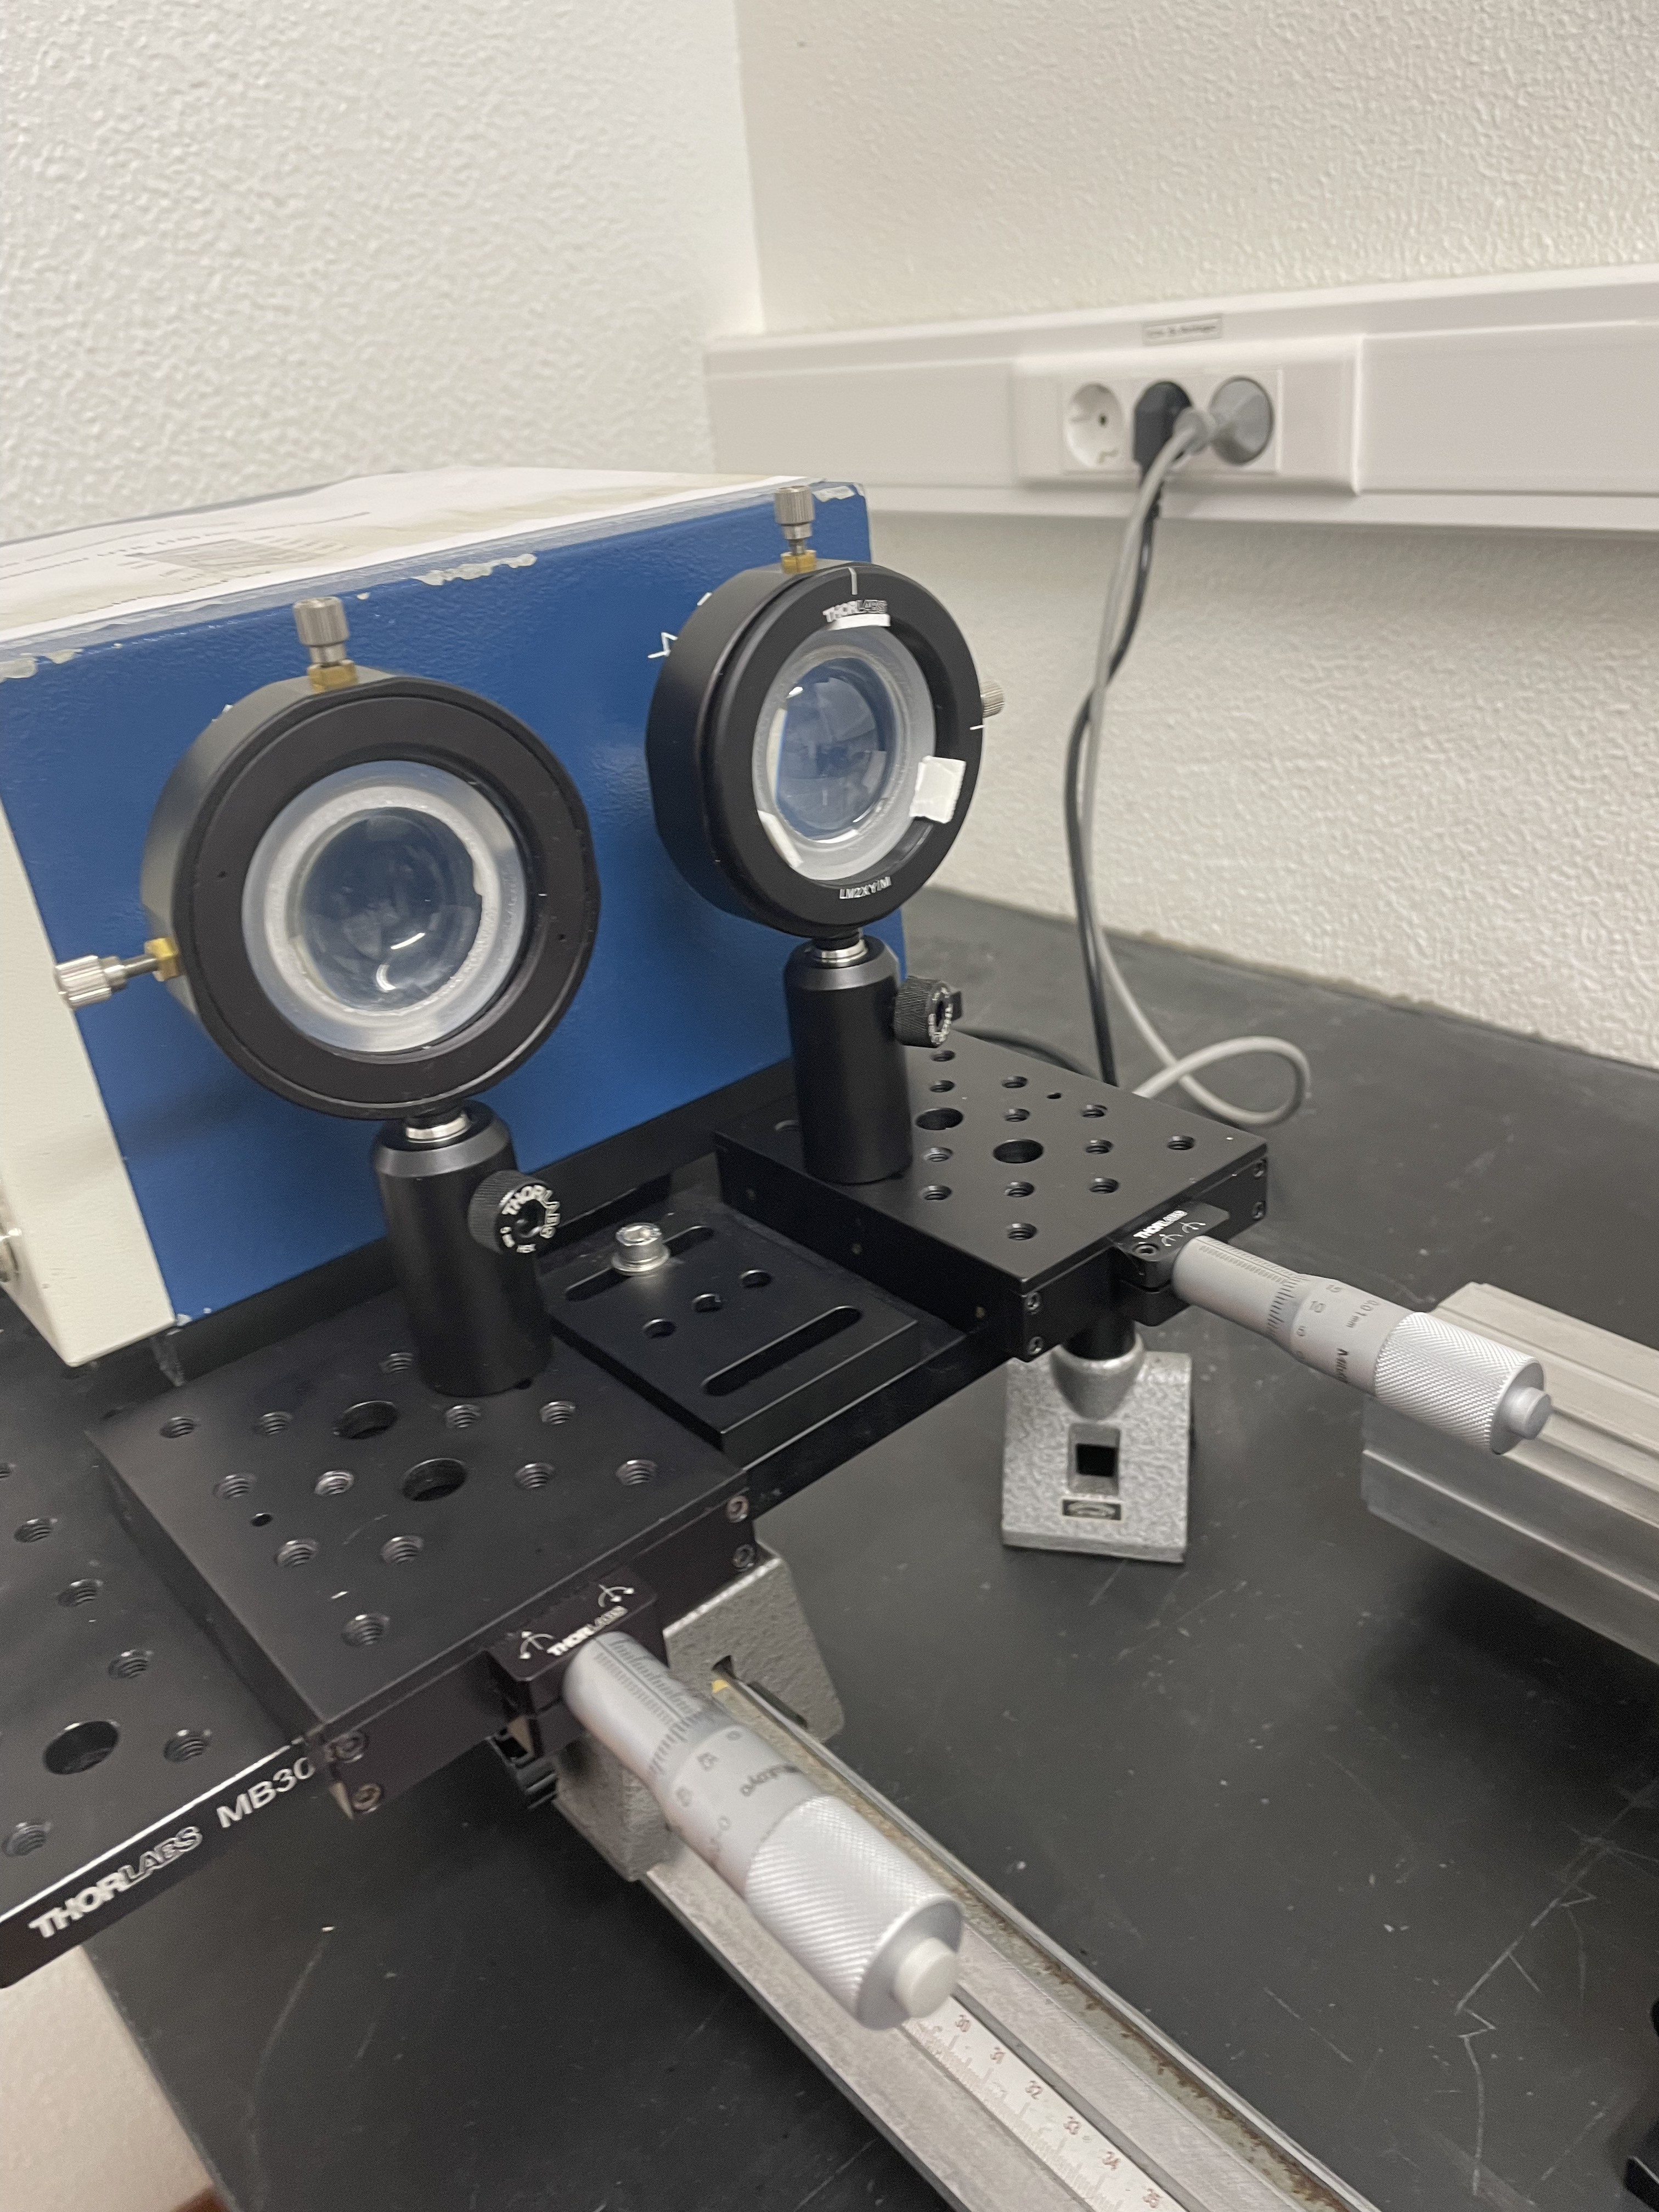
\includegraphics[width=0.6\textwidth]{IMG_2864.jpg}
    \caption{Montagem da experiência com a nova calha e as novas lentes.}
    \label{fig:montagem}
\end{figure}

\begin{figure}[H]
    \centering
    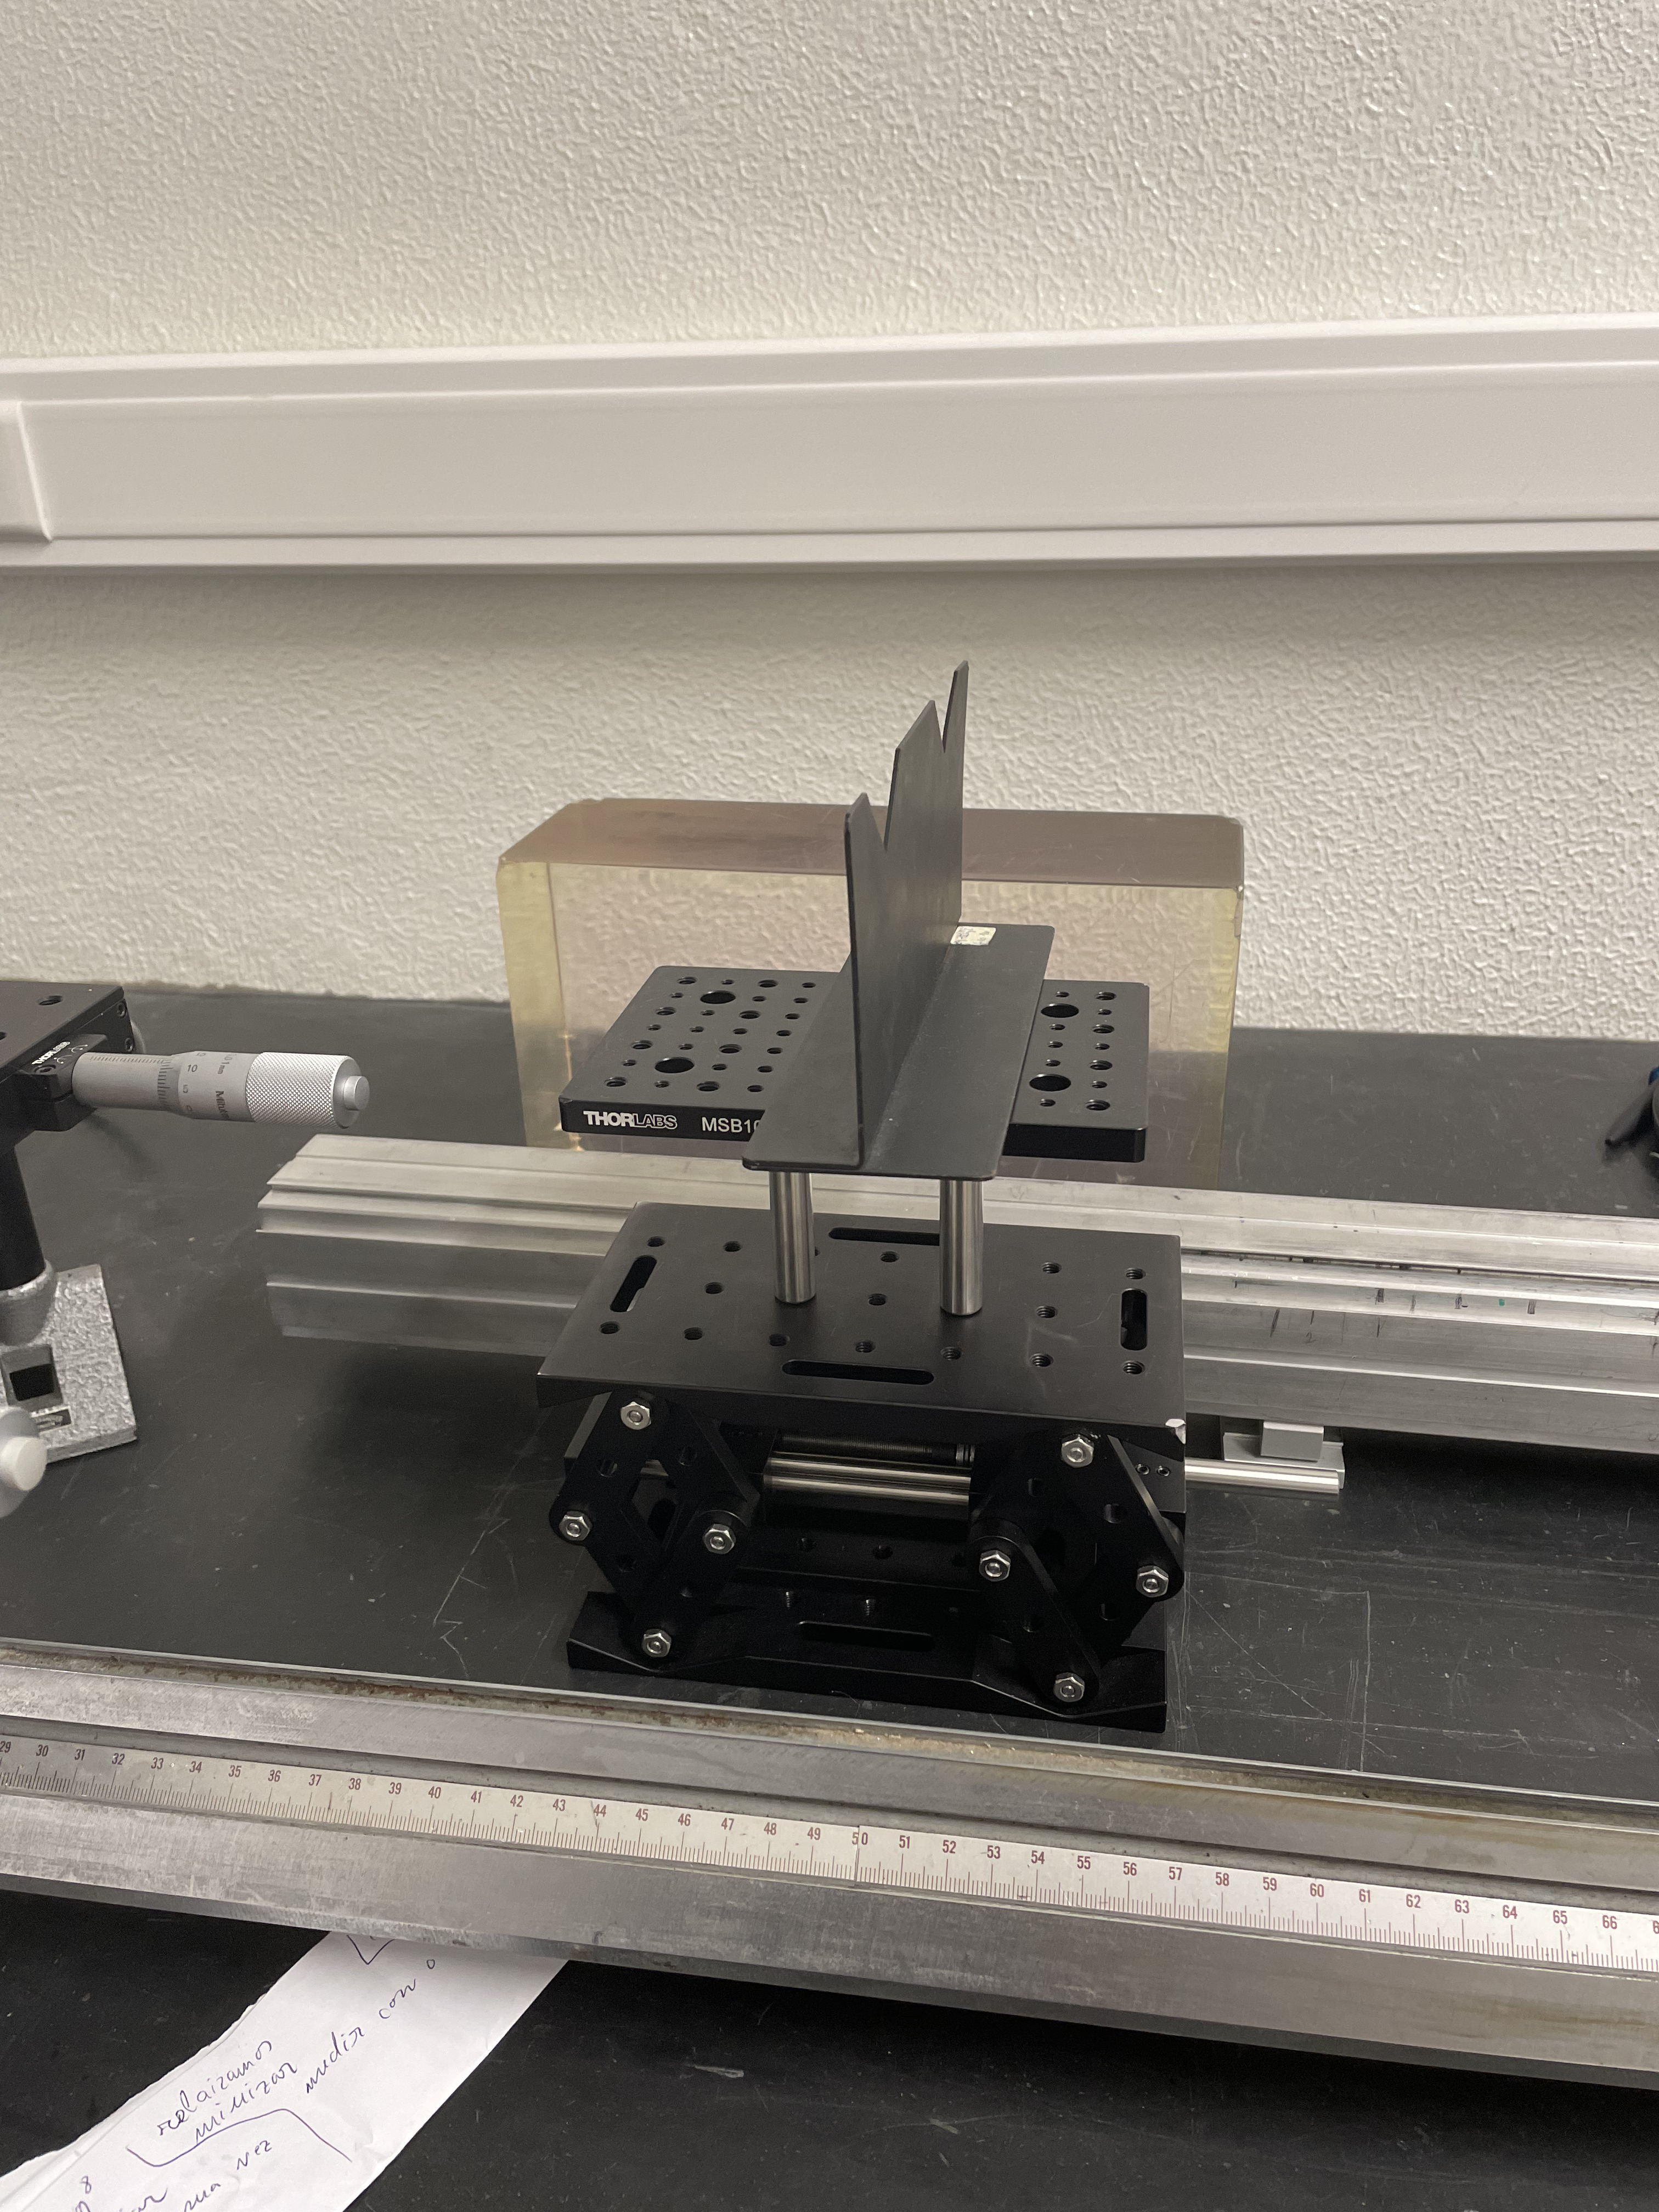
\includegraphics[width=0.6\textwidth]{IMG_2868.jpg}
    \caption{Montagem da experiência com a nova calha e as novas lentes.}
    \label{fig:montagem}
\end{figure}

\begin{figure}[H]
    \centering
    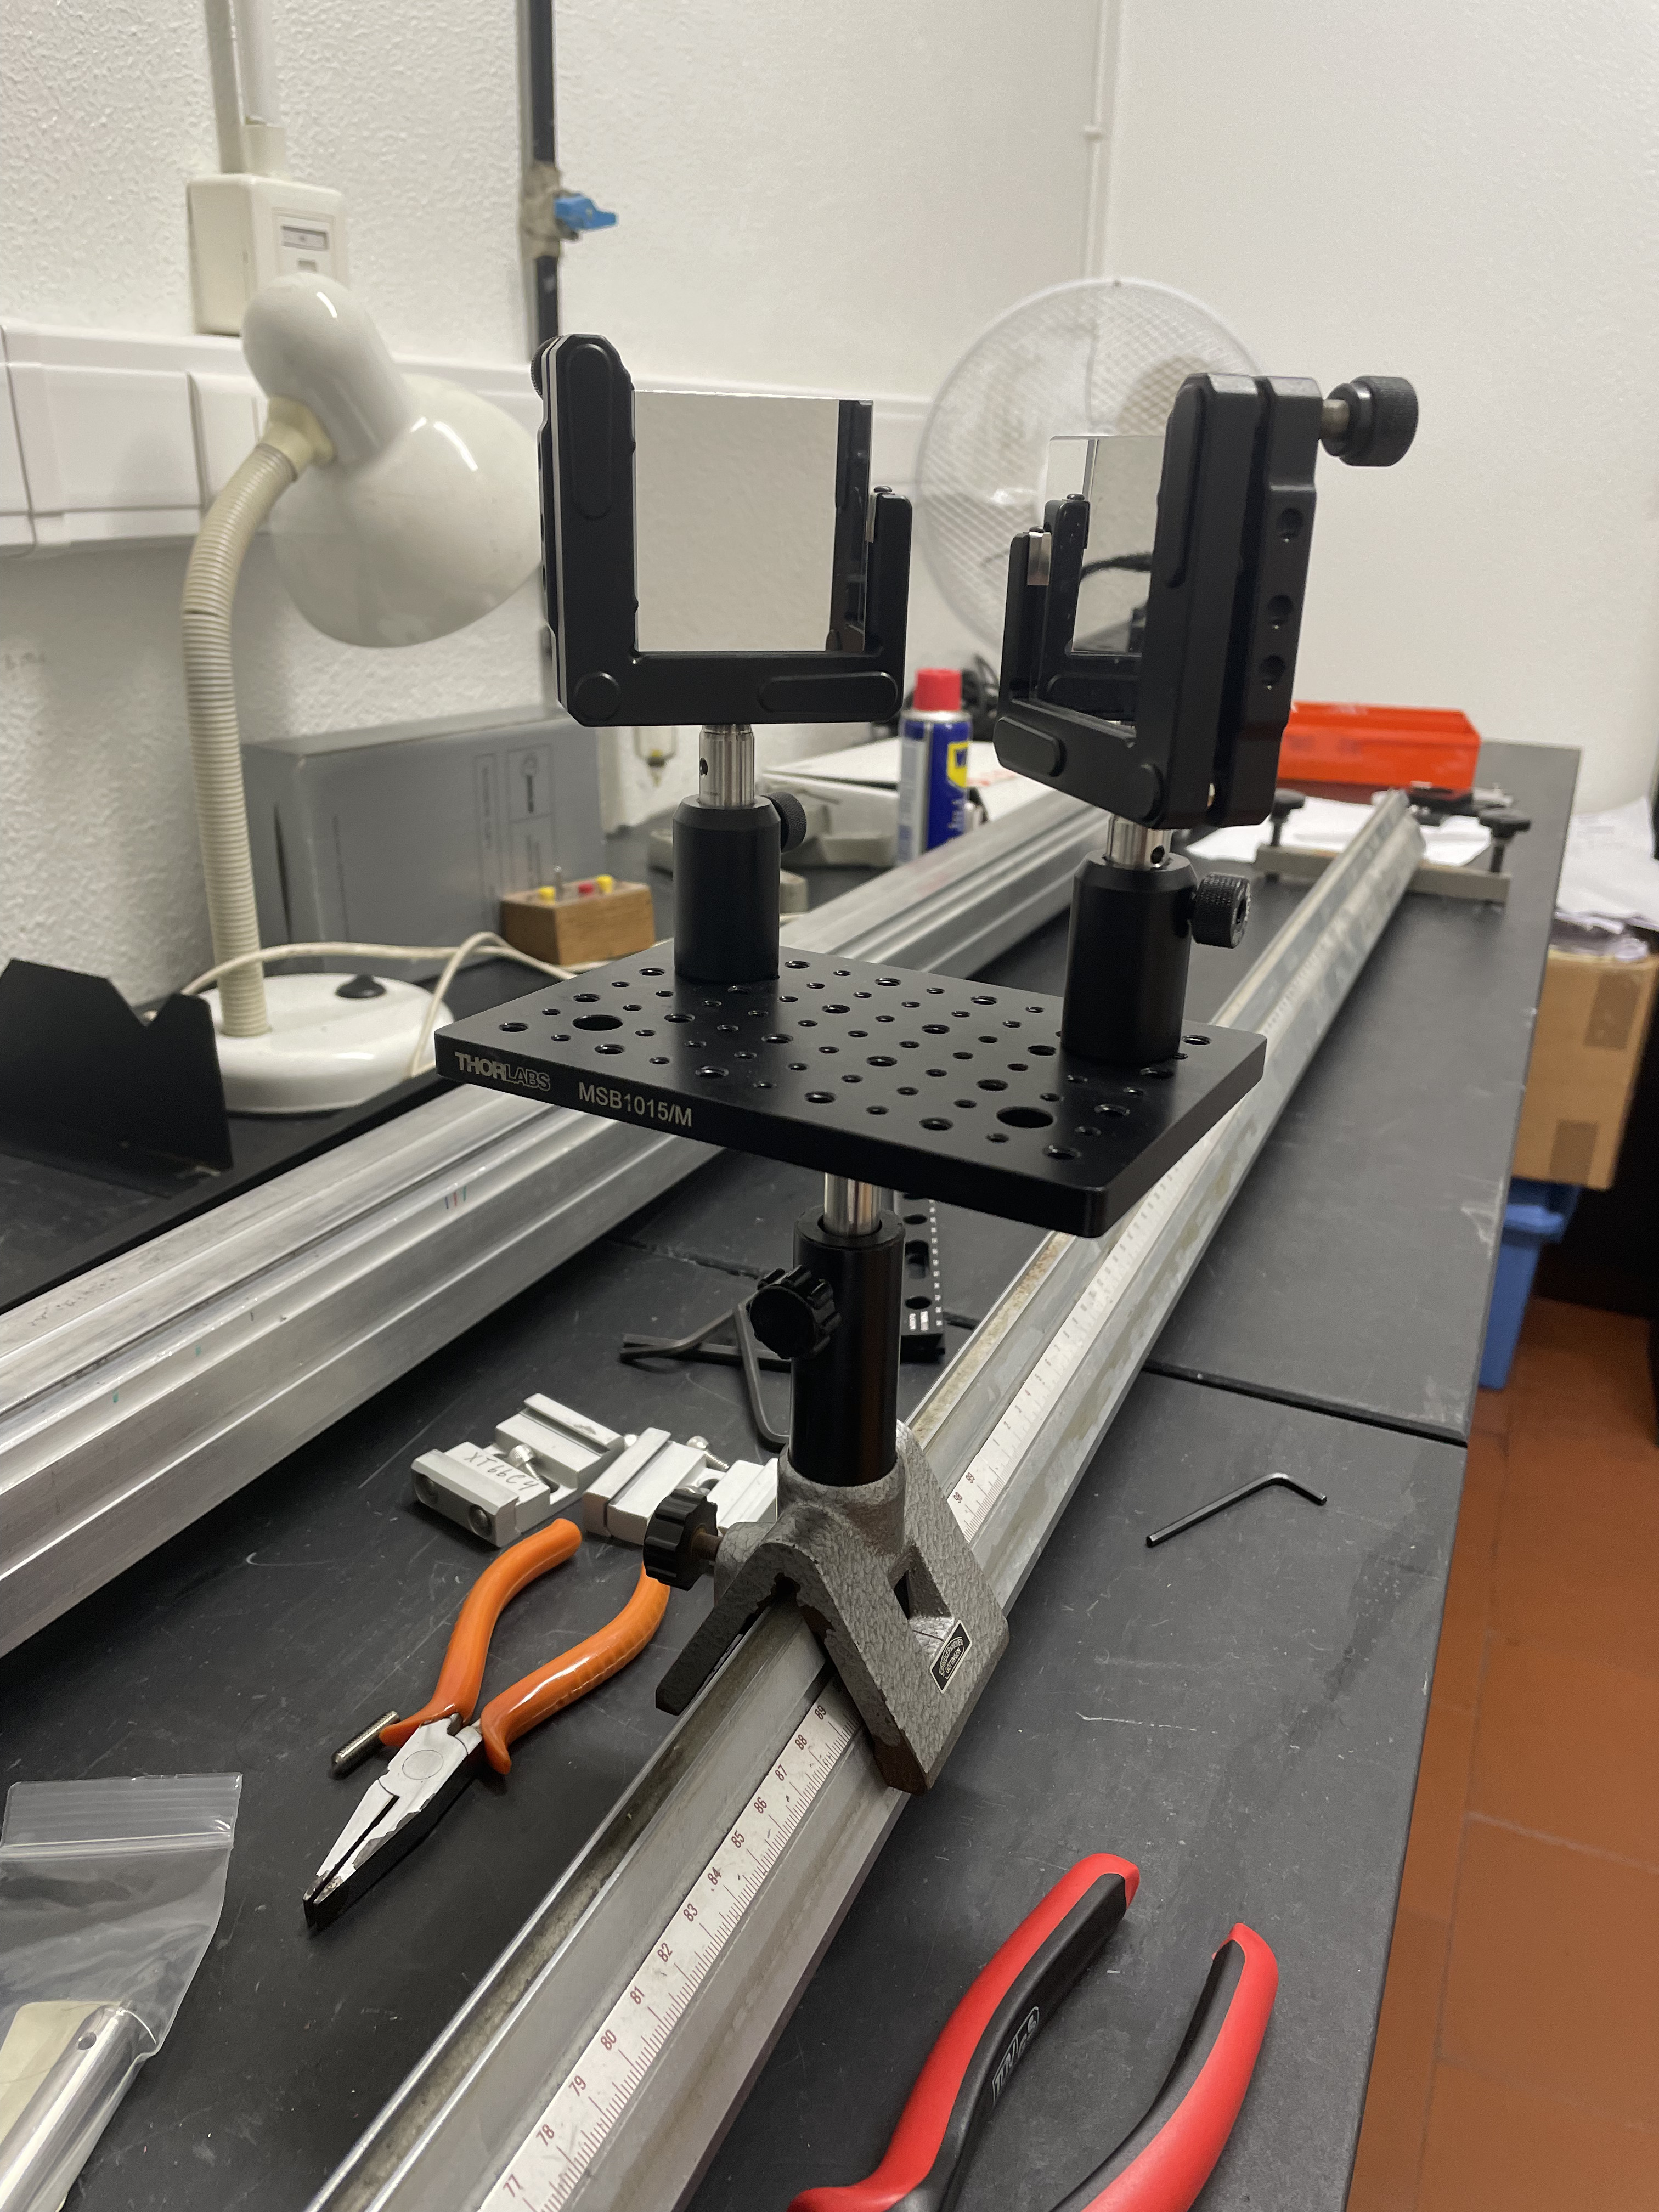
\includegraphics[width=0.6\textwidth]{IMG_2871.jpg}
    \caption{Montagem da experiência com a nova calha e as novas lentes.}
    \label{fig:montagem}
\end{figure}

\begin{figure}[H]
    \centering
    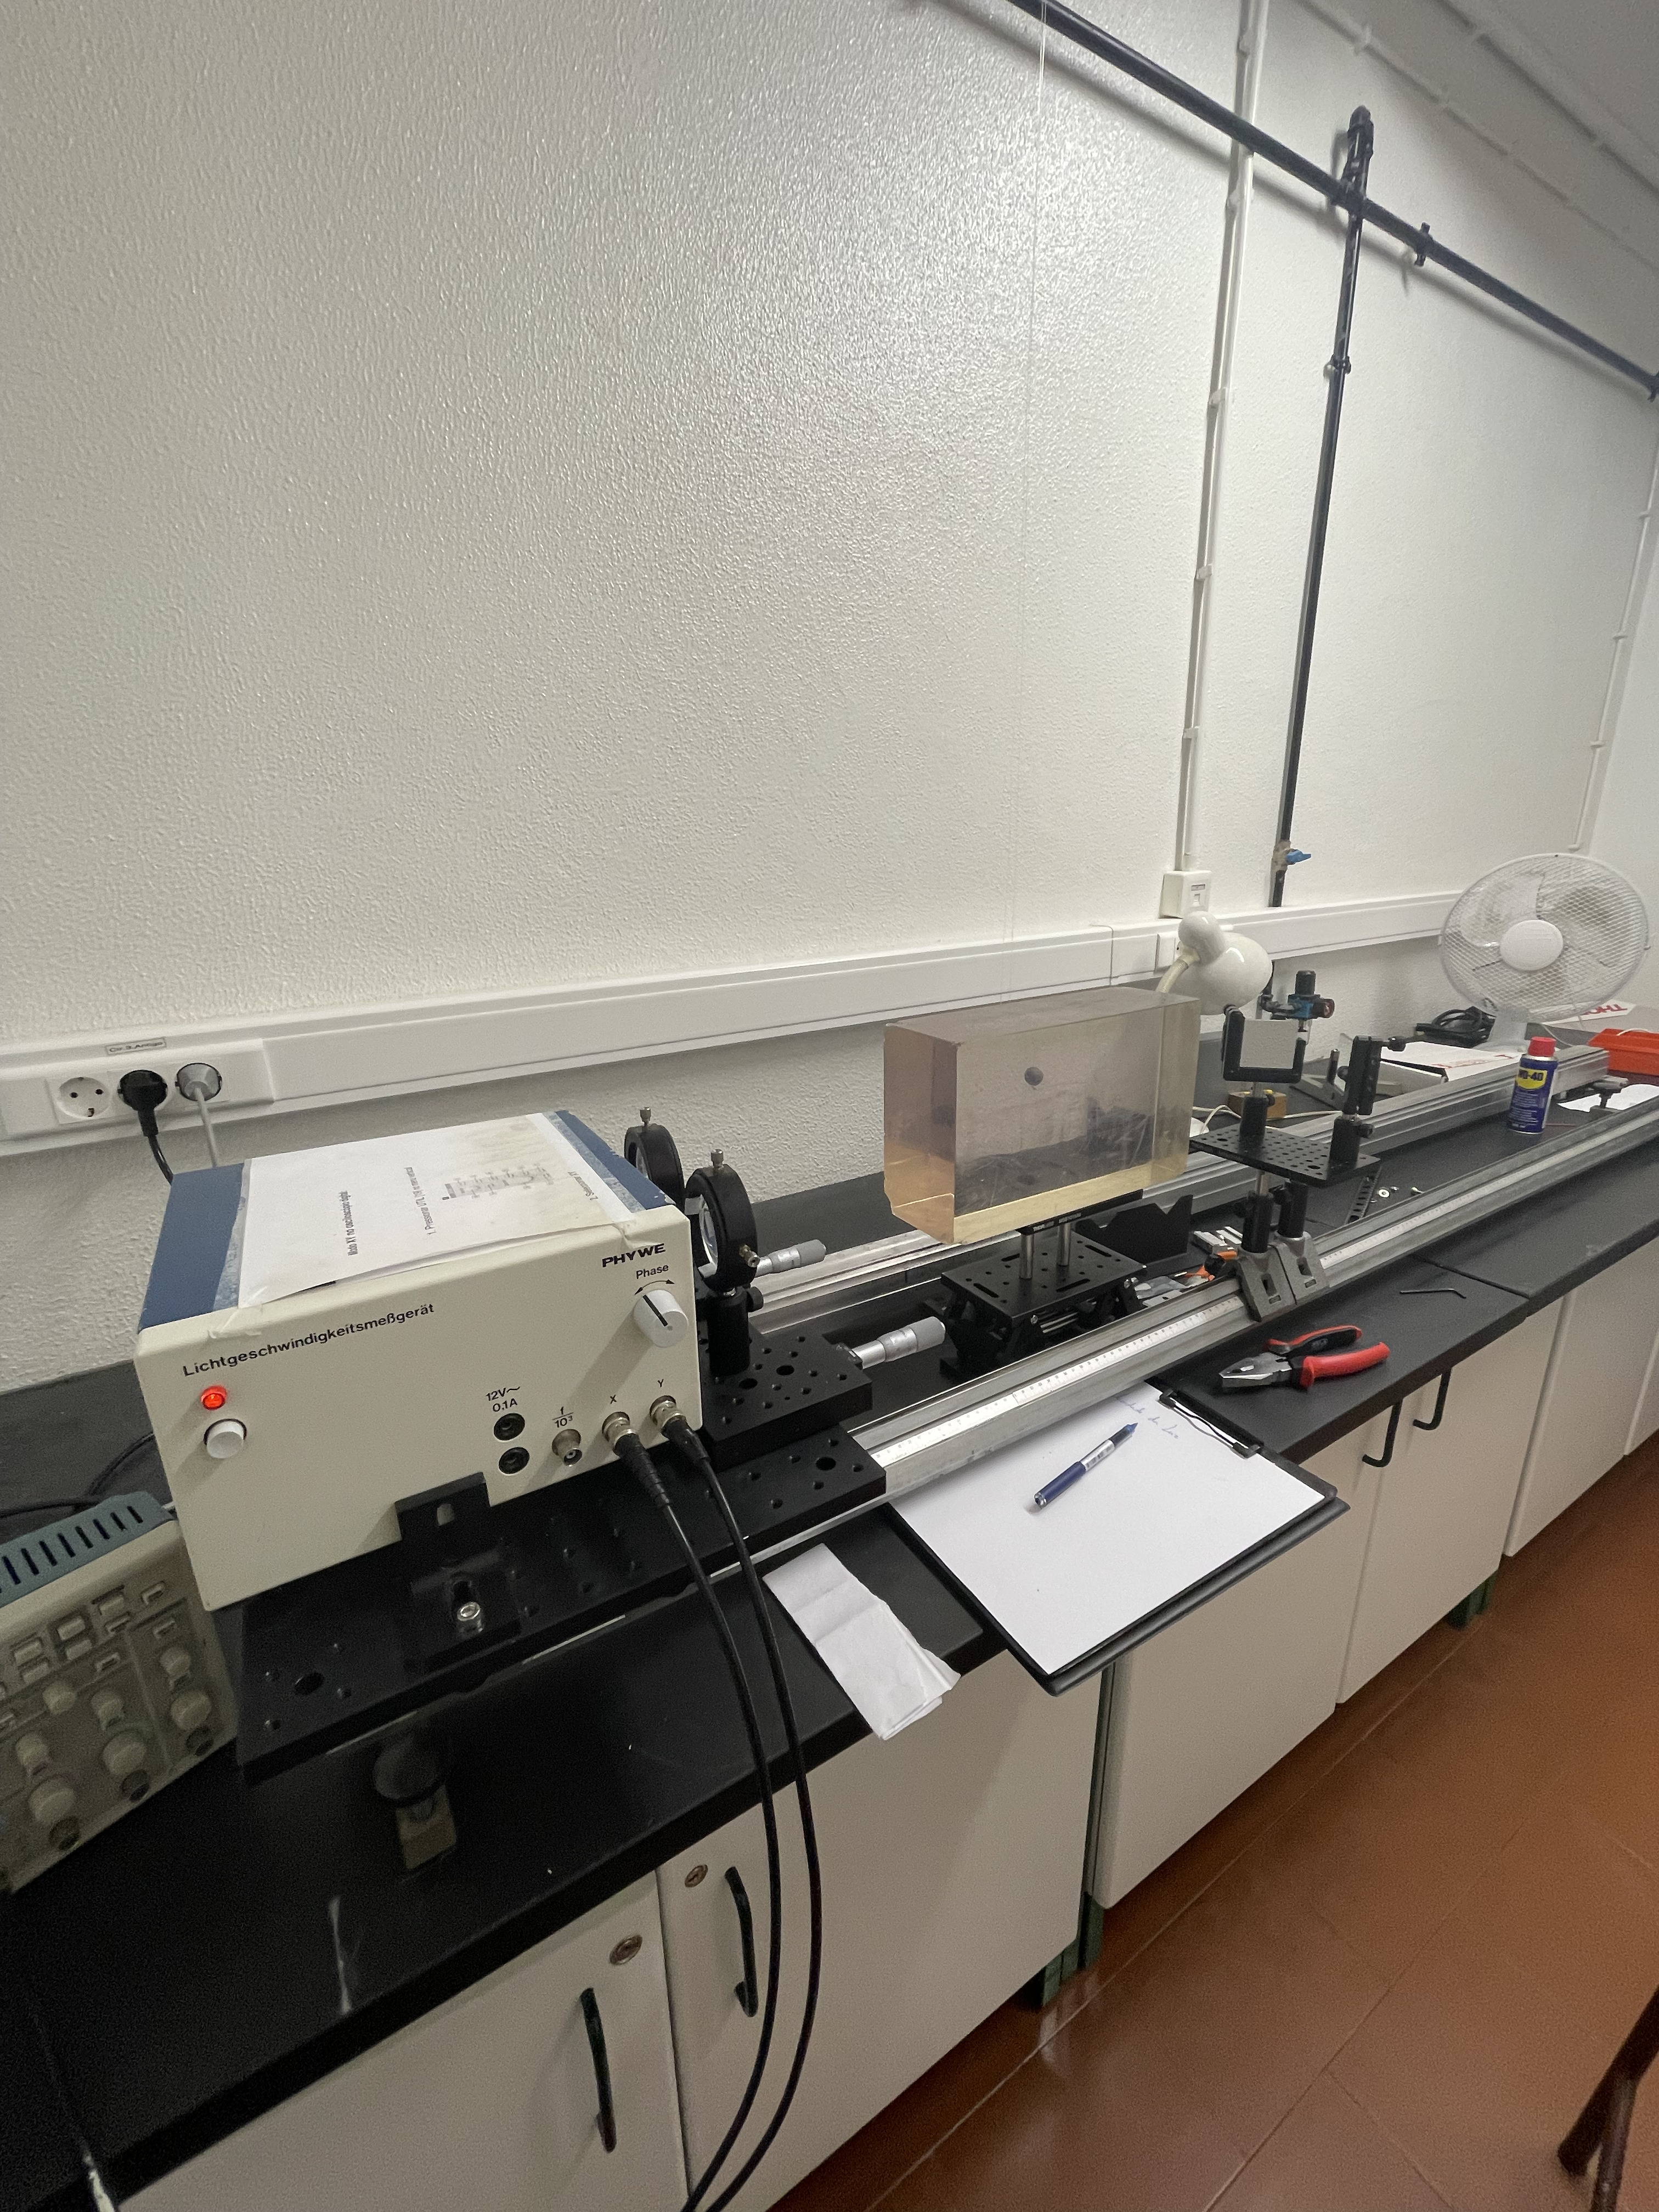
\includegraphics[width=0.6\textwidth]{IMG_2875.jpg}
    \caption{Montagem da experiência com a nova calha e as novas lentes.}
    \label{fig:montagem}
\end{figure}


\newpage

\end{document}

